\chapter{Scaling Throughput in Bitcoin}
The main goal we are seeking to achieve in this chapter and the next following ones is to improve the performance of Bitcoin in different directions. \\
One measurement for the performance of blockchain platforms is the number of transactions per second (tx/s) that they can process. Bitcoin currently has a low tx/s rate, which limits its scalability and usability. Therefore, it is important to find ways to improve Bitcoin’s performance in different dimensions.\\
Some of the dimensions to improve Bitcoin are:
\begin{itemize}
    \item \textbf{Throughput}: how many transactions can be processed in a given period of time.
    \item \textbf{Latency}: how fast a transaction can be confirmed and added to the blockchain.
    \item \textbf{Lightweight}: How much storage, communication, and computation resources are required to run the system?
\end{itemize}
There are two main approaches to improve Bitcoin’s performance: layer one scaling and layer two scaling.\\\\
Layer one scaling refers to modifying the protocol itself, such as increasing the block size, reducing the block interval, or changing the consensus mechanism. These changes can increase the throughput and reduce the latency of Bitcoin, but they may also introduce security and compatibility issues.\\\\
Layer two scaling refers to building solutions on top of the protocol, such as payment channels, sidechains, or sharding. These solutions can enable faster and cheaper transactions without affecting the security and decentralization of Bitcoin, but they may also introduce complexity and interoperability issues.

\section{Bitcoin’s throughput is security limited}
One of the challenges of Bitcoin is its limited transaction throughput. The transaction throughput of Bitcoin depends on two factors:
\begin{itemize}
    \item \textbf{Block size}:  The maximum amount of data that can fit in a block
    \item \textbf{Block interval} : The average time between two consecutive blocks.
\end{itemize} 
Bitcoin can process about 7 transactions per second (tx/s), which is calculated as follows:
\begin{itemize}
    \item A block is 1 MB, which is equivalent to 1,000,000 bytes.
    \item A transaction is about 250 bytes on average.
    \item Therefore, a block can contain about 4,000 transactions (1,000,000 / 250).
    \item A block interval is 10 minutes, which is equivalent to 600 seconds.
    \item Therefore, the transaction throughput is about 7 tx/s (4,000 / 600)
\end{itemize}
We can try increasing the two parameters $\lambda$,$B$ to directly increase throughput:
\begin{itemize}
    \item \textbf{Increasing $\lambda$} directly impacts the security. The hash power of the adversary that can be tolerated
    decreases as $\lambda\Delta$ increases
    \item \textbf{Increasing $B$} proportionally increases the network delay $\Delta$: it takes longer to transmit
    a bigger packet
\end{itemize}
We conclude that the throughput of Bitcoin is limited by security constraints.
Ethereum did it to the extent you thought that you could get away with the security risks.\\\\
To improve Bitcoin’s throughput while keeping its security, three different methods were tried; the first two had some success but not enough, while the third solved the problem completely.
\section{GHOST - embrace forking}
When the mining rate or the block size increases, so does the product of $\lambda$ and $\Delta$. This product is related to the forking rate, which is the percentage of blocks that are left out of the longest chain.\\
A different mining rule that accepts forking (instead of rejecting it like the longest chain protocol) could be better for security. This is the idea behind the GHOST (greedy heaviest observed subtree) fork choice rule:\\
The “quality” of a chain is not measured by its height, but by how heavy the subtree that is linked to it is. That is the main idea.\\\\
The weight of a subtree is the total number of blocks in that subtree, regardless of whether they are valid or not. The rule then selects the chain that has the heaviest subtree as the longest chain.
\begin{figure}[h!]
    \centering
    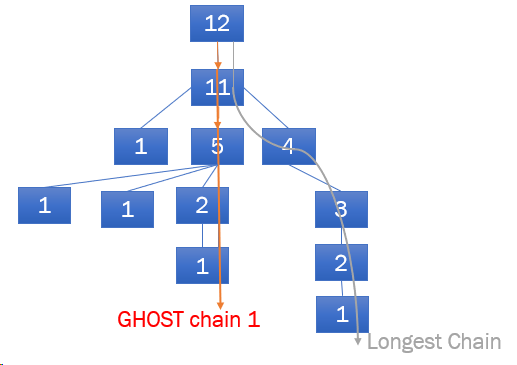
\includegraphics[width=0.5\linewidth]{Fig/08/F1}
    \caption{GHOST chain vs. Longest chain }
    \label{fig:f1}
\end{figure}\\
In Figure \ref{fig:f1}, the weights of the blocks are labeled inside each block. The GHOST chain and the longest chain could be different.
\subsection{Private attack on GHOST}
One of the threats to the security of Bitcoin is a private attack. The GHOST rule claims to be secure against this attack, as long as more than half of the hash power is honest. The reason is that the weight of the honest subtree is proportional to the honest mining rate, while the weight of the private subtree is proportional to the adversary mining rate. Therefore, the honest subtree will always be heavier than the private subtree, and the GHOST rule will choose it as the valid chain. This security guarantee does not depend on the mining rate, so the throughput can be increased by increasing the mining rate, as long as the network can handle it.
\begin{figure}[h!]
    \centering
    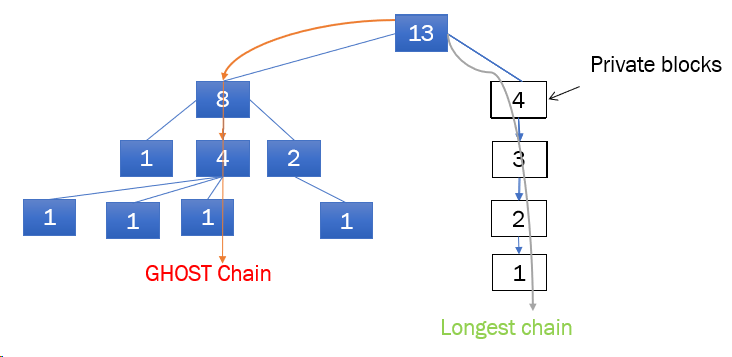
\includegraphics[width=0.6\linewidth]{Fig/08/F2}
    \caption{Private attack in GHOST}
    \label{fig:f2}
\end{figure}\\
Unlike the Longest chain protocol, private attack is no longer the worst-case attack for GHOST rule anymore.
\subsection{Balance attack on GHOST}
The balance attack aims to create two equally weighted chains (based on the GHOST rule) by the adversary. Honest miners choose the oldest chain to mine on when there are multiple chains with the same weight. The adversary can manipulate the network so that each half of the honest nodes sees a different chain first. This way, the honest nodes are divided into two groups, each mining on a different chain, and the adversary can mine privately on both chains from the genesis block (see Figure \ref{fig:f3}). The adversary reveals its blocks as needed (to keep the balance of the two chains). The blockchain protocol becomes unsafe if the balance attack lasts longer than the confirmation depth k.
\begin{figure}[h!   ]
    \centering
    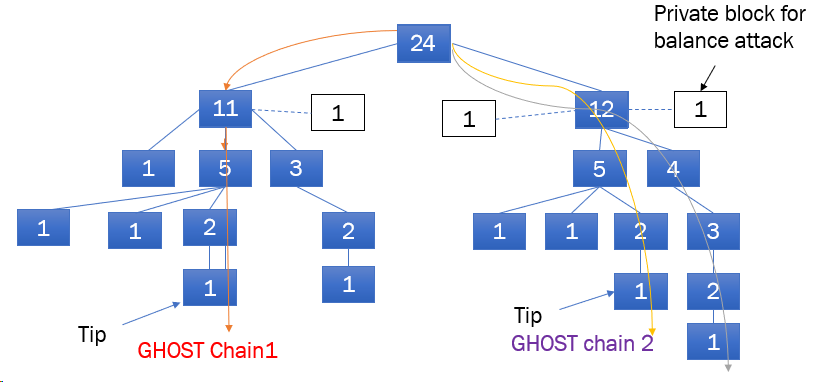
\includegraphics[width=0.7\linewidth]{Fig/08/F3}
    \caption{Balance attack on GHOST}
    \label{fig:f3}
\end{figure}

\section{Reduce Forking and Bitcoin-NG}
One way to reduce forking in the blockchain is to modify the longest chain rule, which states that a miner can only propose one block for each successful nonce. Instead, we could allow a miner to propose multiple blocks for the same nonce, creating a longer chain faster. This would discourage other miners from forking the chain, as they would have to catch up with more blocks. However, this idea is different from simply increasing the block size.\\\\
Bitcoin-NG is based on the idea of dividing the blocks into two parts: a proposer block and a transaction block. The idea is somewhat like the Fruitchains protocol we learned in Chapter 7. This way, the proposer blocks are mined at a low frequency, but the transaction blocks are generated at a high frequency, allowing for faster confirmation and higher throughput of transactions.\\\\
The mining process is as follows:
\begin{itemize}
    \item Unlike Bitcoin, where the miners remain completely anonymous and expose security risks, proposer blocks include the miner’s public key when they are mined.
    \item The transaction blocks are not subject to proof of work and are simply signed (using the private
    key) by the miner whose public key is embedded in the immediately preceding proposer block.
    Since the transaction blocks are not inhibited by proof of work, they can be added to the
    blockchain as quickly as the underlying network can support their reliable broadcast. The
    transaction blocks continue to be mined until a new proposer block appears on the longest
    chain, after which only this new proposer can mine transaction blocks.
    \item Proposer blocks and transaction blocks are interspersed with each other: proposer blocks are
    mined at the tip of the longest chain: the length is only defined via the number of proposer
    blocks in the chain.
\end{itemize}
\begin{figure}[h!]
    \centering
    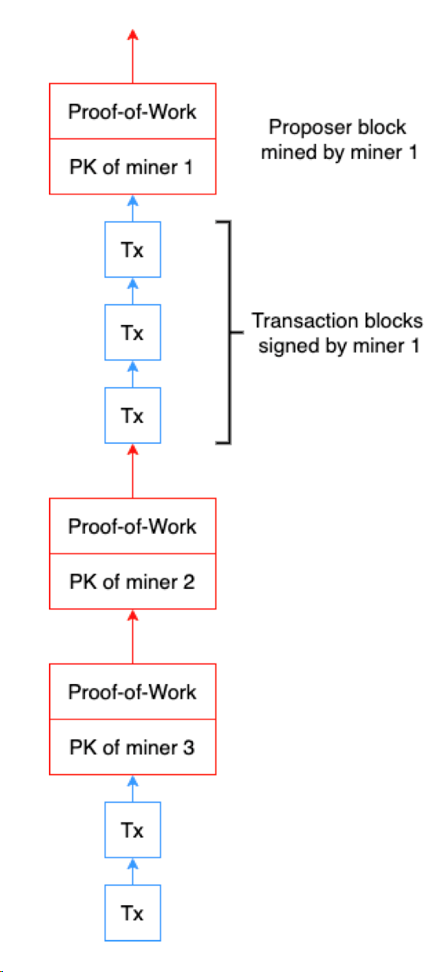
\includegraphics[width=0.3\linewidth]{Fig/08/F4}
    \caption{Bitcoin-NG mining process}
    \label{fig:f4}
\end{figure}
\subsection{Bribing attack in Bitcoin-NG}
A bribing attack on Bitcoin-NG is a type of attack that tries to manipulate the incentives of the miners who create blocks on the blockchain.
 Bitcoin-NG is vulnerable to bribing attacks by an adaptive adversary, who can choose which miners to corrupt while the protocol is running.\\
A bribing attack is a way to incentivize the miners to join the adaptive adversary and collude with them.\\\\
The longest chain protocol has two properties that make it unpredictable and resistant to bribing attacks.
\begin{itemize}
    \item First, no one can know in advance who will mine the next block, or what the contents of the block will be. This makes it hard for an adversary to manipulate the chain or the transactions.
    \item Second, once a block is mined, it is sealed by a nonce and cannot be changed without invalidating the proof-of-work. This makes it costly and risky for an adversary to bribe the miners to alter their blocks.
\end{itemize} 
However, these two properties are only true for proof-of-work (PoW) blocks in Bitcoin-NG. They are not true for transaction (Tix) blocks. Tix blocks are not unpredictable, because they are identified by the public key of the miner in the previous proposer block. Tix blocks are also not sealed, because they can be changed by the miner who has the private key associated with the previous proposer block.\\\\
One example of a bribing attack on Bitcoin-NG is the slow-down attack, which is not a security attack, but a performance attack. The slow-down attack aims to reduce the transaction throughput of Bitcoin-NG by stopping the generation of Tix blocks. The adversary can corrupt the miner who has the latest proposer block on the longest chain, and then bribe them to stop creating Tix blocks. This way, only the transactions in the proposer block will be confirmed, and the throughput will be reduced to the same level as Bitcoin. The slow-down attack can also make it easier for the adversary to perform double-spending attacks because they can create more forks on the chain with fewer Tix blocks.

\section{Prism 1.0 }
Prism 1.0 is a similar protocol to Bitcoin-NG, but it has some differences that make it more secure and efficient. Prism 1.0 also uses two types of blocks: proposer blocks and transaction blocks. However, in Prism 1.0, transaction blocks are not linked to each other or to the proposer blocks. Instead, transaction blocks are referred to as proposer blocks, which means that proposer blocks contain the hashes of transaction blocks. This way, transaction blocks can be created and broadcasted independently, without waiting for the proposer blocks.\\\\
Another difference between Prism 1.0 and Bitcoin-NG is the proof-of-work (PoW) difficulty level for each type of block. In Prism 1.0, transaction blocks have a low PoW difficulty level, which means that they can be mined quickly and easily. This increases the transaction throughput and reduces the latency of the protocol. On the other hand, proposer blocks have a high PoW difficulty level, which means that they are mined infrequently and securely. This ensures the security and stability of the longest chain.\\\\
Prism 1.0 also uses a two-for-one mining procedure and cryptographic sortition to achieve unpredictability and resistance to bribing attacks. Due to the decoupling of transaction blocks from the security of the protocol, the throughput
is only restricted by the capacity of the underlying P2P network. A full-stack UTXO implementation
of Prism achieves more than 70,000 transactions/second.\\\\
The full Prism protocol also resolves another important limitation of the longest chain protocol: latency of
confirmation.
\begin{figure}[h!]
    \centering
    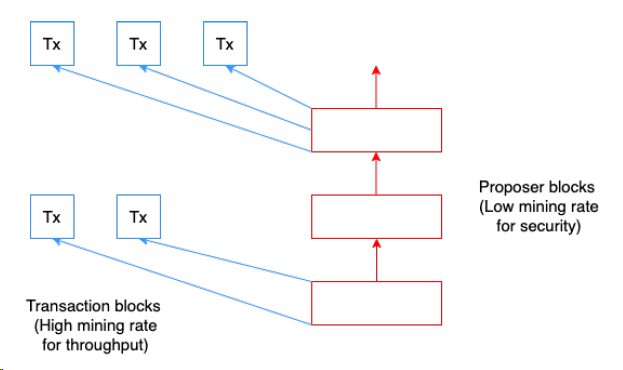
\includegraphics[width=0.5\linewidth]{Fig/08/F5}
    \caption{Prism 1.0 and Fruitchains protocols have two block types: proposer and transaction blocks,
        interspersed with each other. The transaction and proposer blocks are mined in parallel, coupled
        through the sortition process. Transaction block hashes are referred to by proposer blocks thus
        bringing the transactions into the confirmed ledger. Transaction block mining is kept easy (so
        throughput is high) and proposer block mining is kept difficult (so security is high).}
    \label{fig:f5}
\end{figure}

